\documentclass{article}
\usepackage{inputenc, amsmath, hyperref, amsfonts, graphicx, fancyhdr, subfig}

\title{Monotonic Regression Technical Note/ \\ Literature Round-up}
\author{Nathan Willey}
\date{August 2022}

\graphicspath{{./figures/}}

\fancypagestyle{logo}{
	\fancyhf{}
	\fancyhead[LE,LO]{
\includegraphics[scale=.3]{../MTRI_logo.pdf}}}
\pagestyle{logo}

\begin{document}
	
	\maketitle
	
	\section*{Preamble}
	This memo exists as a way for me to summarize my findings about monotonic regression from this summer and provide references to papers in the field that I found to be useful. The hope is that this memo can serve as a helpful launching-off point for a future project in monotonic regression or as a summary of the current landscape. \\
	Thus, here I \textit{quickly} summarize the current state of monotonic regression research and varying implementations. The goal here is for a very broad description, leaving most of the mathematics to the referenced papers. Referenced papers are listed in order of relevance to this memo. \\
	-- Nathan Willey
	
	\newpage
	
	\section*{Methods for Monotonic Regression}
	
	\subsection{i-Splines}
	The first method for monotonic regression, popularized by \ref{iSpline}, uses a monotonically increasing set of basis functions, called i-splines. The basis is defined to be the indefinite integrals of integral-normalized B-splines . It is easy to see these functions are monotonic by the non-negativity of the B-spline basis. These new i-Splines form a basis for the non-decreasing splines of order $k$ when $k \leq 3$ \ref{constrainedSplines}. Furthermore, each function covers the range $[0,1]$ due to the normalization of the B-splines. \\
	
	\begin{figure}[h]
		\label{basisPlots}
		\centering
		\subfloat[\centering]{{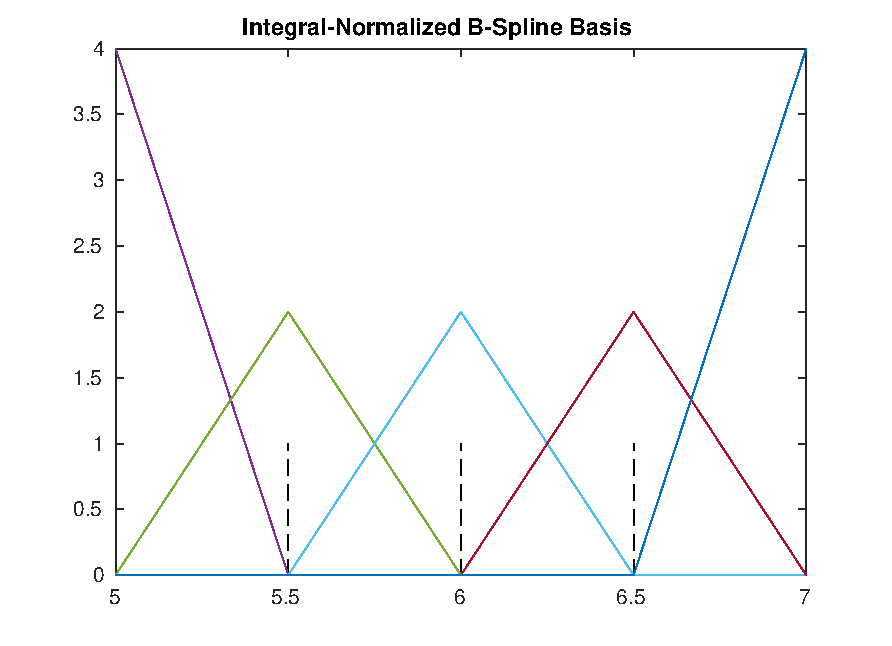
\includegraphics[width=5cm]{msplineBasis.pdf} }}%
		\qquad
		\subfloat[\centering]{{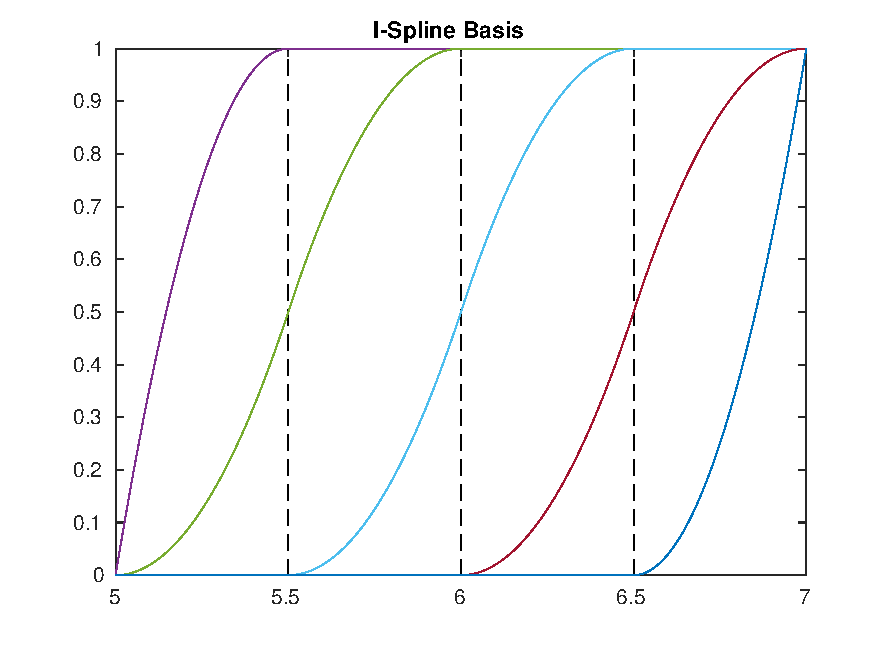
\includegraphics[width=5cm]{isplineBasis.pdf} }}%
		\caption{Integral normalized B-spline basis of order 2 and the respective order 3 i-spline basis acquired by integration of the B-spline basis for 3 inner knots $x \in [5,7]$. \\
		Code to generate basis plots in \textit{nwilley/monotonicReg/ex\_plotSplineBasis.m}}%
		\label{fig:example}%
	\end{figure}
	
	Performing monotonic regression with i-splines follows nearly the same procedure as with b-splines (or any linear basis of functions for that matter), $f(x) = N(x)*\beta$, where $N$ is a matrix holding basis function values at the data points and $\beta$ holds the spline coefficients and is determined to minimize a least squares problem \ref{ESL}. With i-splines, however, it vital to have the restriction $\beta \succeq 0$ to ensure monotonicity.
	
	Due to the fact that each i-Spline basis function covers exactly $[0,1]$, a linear combination s.t. $\beta \in \mathcal{S}_N$ (the N-dimensional probability simplex) gaurentees that $f(0) = 0$ and $f(x_N) = 1$. Thus, with a simplex-restriction on the spline coefficients it is easy to directly fit probability functions with i-splines.
	
	In modern practice, using the basis of quadratic i-splines is probably the most common to fit functions with a continuous derivative. Higher degree i-splines can also be used, but there is no mathematical guarantee that the true minimizer of the non-negative nth degree splines lies in the linear region $\beta \succeq 0$. A very succinct write up explaining the basics of i-splines and how to explicitly compute them is found in \ref{ComputingISpline}. The code detailed there is implemented at \textit{/nwilley/monotonicReg/monotonicRegression.m}
	
	\begin{figure}[h]
		\centering
		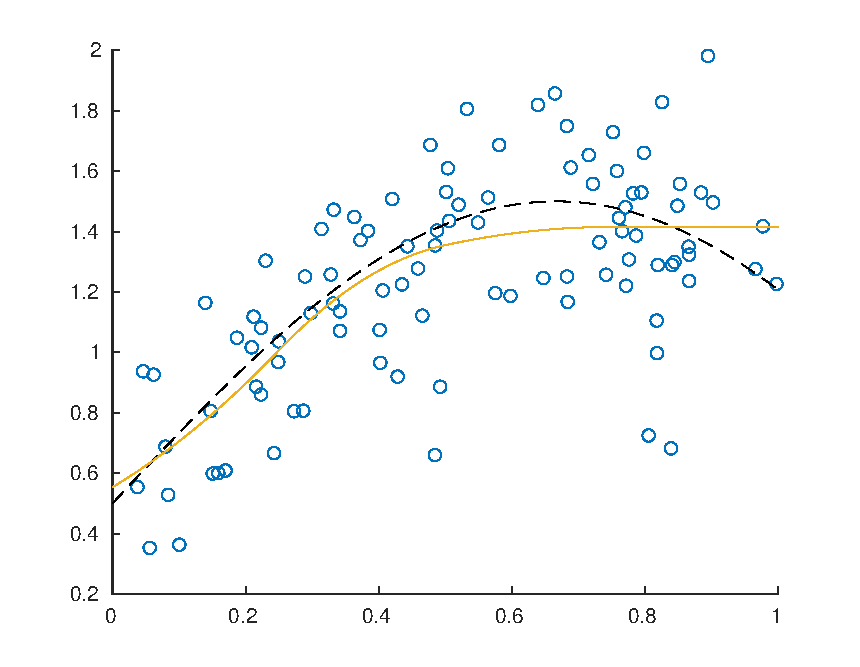
\includegraphics[width=7cm]{sinFit.pdf}
		\caption{$f(x) = \sin(\frac{3pi}{4}x)$ fit using quadratic regression i-splines with 5 knots over the region $[0,1]$. $N=100$. \\ Dashed line shows true function, gold line shows the spline}
	\end{figure}
	
	\subsection{p-Splines}
	
	p-Splines (or penalized splines) are another useful and common tool seen in modern regression splines \ref{pSpline}. The approach here is not limited to monotonic splines, but can be directly utilized in the monotonic case. \\
	p-Splines introduce a discrete penalty on the coefficients of a regression spline to enforce smoothness of varying orders. In practice, impressive results have been obtained with p-splines, with the drawback that the implied definition of smoothness of varying orders is harder to intuit than the usual $\int_a^b |f''|$ penalty.
	
	With a penalty on the spline coefficients, it is feasible to introduce a large number of (equally spaced) knots in order to allow the splines to match the function on highly varying regions, while staying smooth on less varying ones. In practice, letting the number of knots exceeed the number of data points is a very viable approach \ref{pSpline}. \\
	
	Coming back to monotonic regression, implementing a p-spline discrete penalty into the i-spline regime allows for an almost non-parametric, monotonic fit. Coupled with the previously mentioned simplex-restriction on $\beta$, this gives a direct way to spline a probability function, with user-control over smoothness. This is also implemented currently in \textit{/nwilley/monotonicReg/monotonicRegression.m}
	
	\begin{figure}[h]
		\centering
		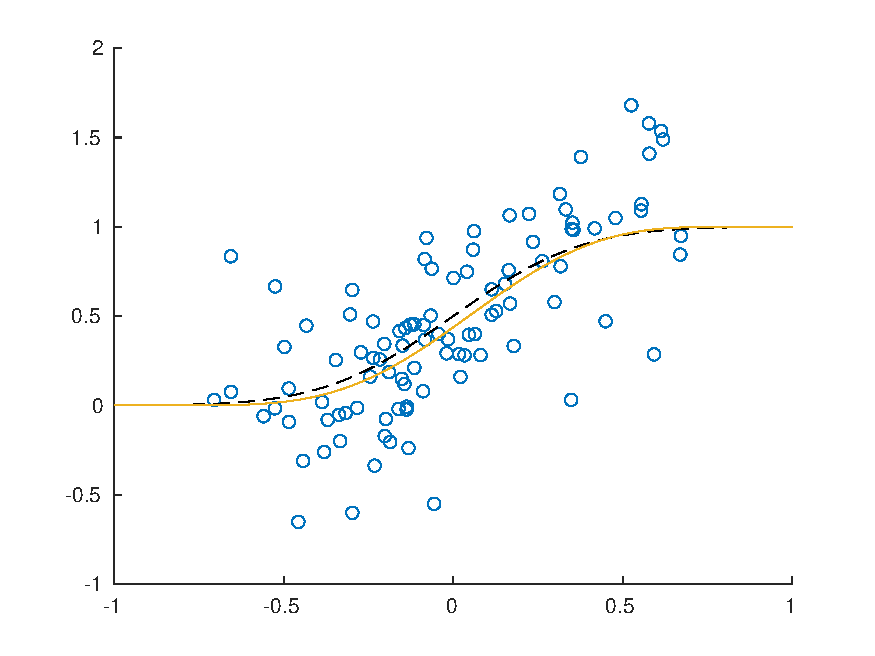
\includegraphics[width=7cm]{normalcdfFit.pdf}
		\caption{Non-parametric quadratic i-spline fit of a Gaussian cdf $(\mu, \sigma) = (0, 0.3)$ using second order p-spline penalty and a probability function restriction on $\beta$. $N=100$, data has Gaussian error around the true distribution, and 100 knots are placed in the region $[-1,1]$}
	\end{figure}

	\subsection{Monotonic Cubic Smoothing Splines and SOCP}	
	
	Finally, I want to mention another approach that has been taken to monotonic regression. \ref{SOCPSpline} directly finds a way to compute \textit{cubic smoothing splines} (knot at every data point) with monotonicity restrictions. The idea here is that they turn the problem into a second-order cone optimization problem (SOCP), allowing direct minimization of a traditional cubic spline enforcing necessary and sufficient conditions for monotonicity. \\
	This approach is more complex than the i-spline approach, but gives a direct analogue to cubic smoothing splines with monotonicity. In practice, this method performs similarly to regression i-splines. Furthermore, this method does not have a clear way to enforce probability curve restrictions on the resulting spline, unlike i-splines. Thus, this approach may prove more useful if implemented in traditional monotonic problems, but lack benefits over non parametric i-splines for fitting probability curves.
	\newpage
	
	\begin{thebibliography}{9}
		\bibitem{iSpline}
		\label{iSpline}
		Ramsay, James O. "Monotone regression splines in action." Statistical science (1988): 425-441.
		
		\bibitem{ComputingISpline}
		\label{ComputingISpline}
		de Leeuw, J. (2017). Computing and fitting monotone splines. University of California, Los Angeles.
		
		\bibitem{pSpline}
		\label{pSpline}
		Eilers, P. H., Marx, B. D. (1996). Flexible smoothing with B-splines and penalties. Statistical science, 11(2), 89-121.
		
		\bibitem{SCOPSpline}
		\label{SOCPSpline}
		Wang, X., Li, F. (2008). Isotonic smoothing spline regression. Journal of Computational and Graphical Statistics, 17(1), 21-37.
		
		\bibitem{constrainedSplines}
		\label{constrainedSplines}
		Meyer, Mary C. "Constrained penalized splines." Canadian Journal of Statistics 40.1 (2012): 190-206.
		
		\bibitem{ESL}
		\label{ESL}
		Hastie, T., Tibshirani, R., Friedman, J. H., Friedman, J. H. (2009). The elements of statistical learning: data mining, inference, and prediction (Vol. 2, pp. 1-758). New York: springer.
		

		
	\end{thebibliography}
	
\end{document}
	
	
	
	
	
	
	